\documentclass[11pt]{article}
\usepackage{graphicx}
\DeclareGraphicsRule{.tif}{png}{.png}{`convert #1 `dirname #1`/`basename #1 .tif`.png}

\textwidth = 6.5 in
\textheight = 9 in
\oddsidemargin = 0.0 in
\evensidemargin = 0.0 in
\topmargin = 0.0 in
\headheight = 0.0 in
\headsep = 0.0 in
\parskip = 0.2in
\parindent = 0.0in
\usepackage{paralist} %compactenum

%\newtheorem{theorem}{Theorem}
%\newtheorem{corollary}[theorem]{Corollary}
%\newtheorem{definition}{Definition}
\usepackage{tipa}
\usepackage{amsfonts}
\usepackage[mathscr]{eucal}

% Use the natbib package for the bibliography
\usepackage[round]{natbib}
\bibliographystyle{apalike}
\newcommand{\exampleMacro}[1]{\mu_{#1}}

\title{Brief Article}
\author{The Author}

\usepackage{url}
\usepackage{hyperref}
\hypersetup{backref,  pdfpagemode=FullScreen,  linkcolor=blue, citecolor=red, colorlinks=true, hyperindex=true}

\begin{document}
You suspect that a population of big horn sheep are made up of two classes of males based on their sparring ability: Strong and Weak. The proportion of strong individuals is unknown.\\ {\bf Experiment:}
\begin{compactitem}
	\item You randomly select 10 pairs of males from a large population. 
	\item For each pair you randomly assign one of them the ID 0 and the other the ID 1.  
	\item You record the \# of winner from 2 contests.
\end{compactitem}
{\bf Model:}
\begin{compactitem}
	\item If two individuals within the same class fight, you expect either outcome to be equally likely.
	\item If a Strong is paired against a Weak then you expect that the probability that the stronger one wins with some probability, $w$.
	\item $w$ is assumed to be the same for every pairing of Strong {versus} Weak and the same for every bout within such a pairing.
\end{compactitem}
Here is the data (and three alternative codings):\\
\begin{center}
\begin{tabular}{|c|c|c|}
\hline
& \multicolumn{2}{c|}{winner}\\
Pair \# & bout 1 & bout 2 \\
\hline
1 & 1 & 1  \\
\hline
2 & 1 & 0  \\
\hline
3 & 0 & 1  \\
\hline
4 & 1 & 1  \\
\hline
5 & 0 & 0  \\
\hline
6 & 0 & 1   \\
\hline
7 & 1 & 1  \\
\hline
8 & 0 & 0  \\
\hline
9 & 1 & 0  \\
\hline
10 & 1 & 1   \\
\hline
\end{tabular}
\begin{tabular}{|lc|}
\hline
& \\
\multicolumn{2}{|c|}{$X$}\\
\hline
$x_1 = 1$ & $x_{11} = 1$  \\
$x_2 = 1$ & $x_{12} = 0$  \\
$x_3 = 0$ & $x_{13} = 1$  \\
$x_4 = 1$ & $x_{14} = 1$  \\
$x_5 = 0$ & $x_{15} = 0$  \\
$x_6 = 0$ & $x_{16} = 1$  \\
$x_7 = 1$ & $x_{17} = 1$  \\
$x_8 = 0$ & $x_{18} = 0$  \\
$x_9 = 1$ & $x_{19} = 0$  \\
$x_{10} = 1$ & $x_{20} = 1$  \\
\hline
\end{tabular}
\begin{tabular}{|l|}
\hline
\\
$Y$\\
\hline
$y_1 = (1, 1)$   \\
$y_2 = (1, 0)$  \\
$y_3 = (0, 1)$  \\
$y_4 = (1, 1)$  \\
$y_5 = (0, 0)$  \\
$y_6 = (0, 1)$  \\
$y_7 = (1, 1)$  \\
$y_8 = (0, 0)$  \\
$y_9 = (1, 0)$  \\
$y_{10} = (1, 1)$  \\
\hline
\end{tabular}
\begin{tabular}{|l|}
\hline\\
$Z$\\
\hline$z_1 = 0$   \\
$z_2 = 1$  \\
$z_3 = 1$  \\
$z_4 = 0$  \\
$z_5 = 0$  \\
$z_6 = 1$  \\
$z_7 = 0$  \\
$z_8 = 0$  \\
$z_9 = 1$  \\
$z_{10} = 0$  \\
\hline\end{tabular}

\end{center}
What can we say about $w$?

At first it is tempting to think of this as twenty separate data points, represented by $X$.
We would like to formulate a likelihood:
$$L(w) = \Pr(X|w) = \prod_{i=1}^{n}\Pr(x_i|w)$$
Because our assignment of 0 or 1 to the males is random, we would be forced to conclude that $\Pr(X=0) = \Pr(X=1) = \frac{1}{2},$ and thus the likelihood would be:
\begin{eqnarray*} 
	L(w) & = & \prod_{i=1}^{n}\Pr(x_i|w) \\
	& = & \prod_{i=1}^{20}\frac{1}{20} =  2^{-20}
\end{eqnarray*} 
This is alarming because the likelihood is not a function of $w$.  
If we had done everything right, then such a likelihood would mean that we can infer {\em nothing} about $w$ from these data (every value of $w$ would return the same likelihood).

While it is true that $\Pr(x_1=0)=0.5$, further reflection reveals that $\Pr(x_{11}=0)$ is not necessarily 0.5.  
The outcome of the first bout will give us some information about which male is stronger, and so the outcome of the second bout is not independent of the first bout.
We could approach the likelihood as:
\begin{eqnarray*} 
	L(w) & = & \prod_{i=1}^{10}\Pr(x_i|w)\Pr(x_{i+10}|w)
\end{eqnarray*} 
Where the $i+10$ indexing exploits the fact that I've numbered the subscripts of $x$ such that the $i+10$ datum is the second bout associated with pair $i$.
This is a fine way to proceed, but it may be less clumsy to simply recode the data to reflect that we have a pair of observations.
This is accomplished in the coding referred to as $Y$.  
Now we have ten independent trials, and each realization of the random variable can assume one of four values (this is basically the same as the last likelihood, but we won't be relying on any tricks of variable subscripting).
\begin{eqnarray*} 
	L(w) & = & \prod_{i=1}^{10}\Pr(y_i|w)
\end{eqnarray*}

At this point, we need to think about how to model $\Pr(y_i|w)$ statements.
Let's tackle the probability that we would get a (0,0) outcome from a pair of bouts.
We don't know whether either of the males is ``Strong'' or ``Weak,'' so we'll have to consider all possibilities.
Let's use $r_0$ and $r_1$ to denote the ``class'' of rams 0 and 1; we will allow these variables to be $S$ or $W$ for strong and weak.
By the law of total probability:
\begin{eqnarray*} 
 \Pr(y_i = (0,0)|w)  & = & \Pr(y_i = (0,0)|w,r_0=S,r_1=S)\Pr(r_0=S,r_1=S) + \ldots \\
 & & \ldots + \Pr(y_i = (0,0)|w,r_0=S,r_1=W)\Pr(r_0=S,r_1=W) + \ldots \\
 & & \ldots + \Pr(y_i = (0,0)|w,r_0=W,r_1=S)\Pr(r_0=W,r_1=S) + \ldots \\
 & & \ldots + \Pr(y_i = (0,0)|w,r_0=W,r_1=W)\Pr(r_0=W,r_1=W) \\
\end{eqnarray*}
We note that if the males are evenly matched, then all four values of $y_i$ are equally likely (probability = 1/4).
If we knew the males were mismatched, then the stronger would win both bouts with probability $w^2$ because we assume that the bouts are independent.
The weaker would win both bouts with probability $(1-w)^2$ by the same logic. This leads us to:
\begin{eqnarray*} 
 \Pr(y_i = (0,0)|w)  & = &   \left(\frac{1}{4}\right)\Pr(r_0=S,r_1=S) + w^2 \Pr(r_0=S,r_1=W) + \ldots \\
 &  & \ldots + (1-w)^2\Pr(r_0=W,r_1=S) + \left(\frac{1}{4}\right)\Pr(r_0=W,r_1=W) \\
\end{eqnarray*}

Clearly, if we want to get a likelihood (as a number, not an abstract equation), we'll need to model the probability of each male being strong or weak. 
The problem says that the ``proportion of strong individuals is unknown.''
We can simply treat this as a nuisance parameter, $s$.
Because we are sampling the males randomly, we have:
\begin{eqnarray*} 
 \Pr(y_i = (0,0)|w)  & = &   \left(\frac{1}{4}\right)s^2 + w^2 s(1-s)  + (1-w)^2(1-s)s + \left(\frac{1}{4}\right)(1-s)^2 \\
	 & = &   \left(\frac{1}{4}\right)(1-2s +2s^2) + (1 -2w +2w^2) s(1-s)
\end{eqnarray*}
This does not look too attractive, but we seem to be making progress. We can go through the same steps for the (1,1) outcome, and we get the same functional form:
\begin{eqnarray*} 
 \Pr(y_i = (1,1)|w)  & = &   \left(\frac{1}{4}\right)(1-2s +2s^2) + (1 -2w +2w^2) s(1-s).
\end{eqnarray*}
This makes sense, because we are randomly choosing a male to label 0, so we would not expect the (0,0) outcome to be more probable than the (1,1) outcome.

When we consider an outcome like (0,1), and we have a pairing of males with mismatched strength we find that the probability of the outcome is $w(1-w)$:
\begin{eqnarray*} 
 \Pr(y_i = (0,1)|w)  & = &   \left(\frac{1}{4}\right)s^2 + w(1-w) s(1-s)  + (1-w)w(1-s)s + \left(\frac{1}{4}\right)(1-s)^2 \\
	 & = &   \left(\frac{1}{4}\right)(1-2s +2s^2) + 2w(1-w) s(1-s) \\
\Pr(y_i = (1,0)|w)  & = &\left(\frac{1}{4}\right)(1-2s +2s^2) + 2w(1-w) s(1-s)
\end{eqnarray*}
Adding up all four probabilities gives:
\begin{eqnarray*} 
\mbox{sum} & = & 4\left(\frac{1}{4}\right)(1-2s +2s^2) + 4w(1-w) s(1-s) + 2 (1 -2w +2w^2) s(1-s)\\
& = & (1-2s +2s^2) + s(1-s)\left[4w -4w^2 + 2 -4w +4w^2\right]\\
& = & 1-2s +2s^2 + 2s(1-s)\\
& = & 1-2s +2s^2 + 2s- 2s^2\\
& = & 1
\end{eqnarray*}
which should be the case because probability of all of the distinct events should add up to 1.

We are ready to express the log-likelihood. We will use $n_{00}, n_{01}, n_{10}$, and $n_{11}$ to denote the number of trials that result in $(0,0), (0,1), (1,0)$, and $(1,1)$ respectively:
\begin{eqnarray*} 
\ln L(w,s) & = & n_{00}\ln\left[\left(\frac{1}{4}\right)(1-2s +2s^2) + (1 -2w +2w^2) s(1-s)\right] + \ldots \\
	& & +  n_{01}\ln\left[\left(\frac{1}{4}\right)(1-2s +2s^2) + 2w(1-w) s(1-s)\right] + \ldots \\
	& & +  n_{10}\ln\left[\left(\frac{1}{4}\right)(1-2s +2s^2) + 2w(1-w) s(1-s)\right] + \ldots \\
	& & + n_{11}\ln\left[\left(\frac{1}{4}\right)(1-2s +2s^2) + (1 -2w +2w^2) s(1-s)\right] + \ldots \\
\end{eqnarray*}
\subsection{Sufficiency}
Notice that some of the terms are very similar to each other. This is not surprising, as we noted symmetry before that cause some probabilities to be equal. But it will let us collapse terms:
\begin{eqnarray*} 
\ln L(w,s) & = & (n_{00} + n_{11})\ln\left[\left(\frac{1}{4}\right)(1-2s +2s^2) + (1 -2w +2w^2) s(1-s)\right] + \ldots \\
	& & +  (n_{01}+n_{10})\ln\left[\left(\frac{1}{4}\right)(1-2s +2s^2) + 2w(1-w) s(1-s)\right] \\
\end{eqnarray*}
Recall that the variables with $n$ are the counts that we get from our data and everything else is a parameter.
We have just collapsed terms that feature aspects of our data into a sum.
The fact that we can do this means that $n_{00} + n_{11}$ tells us just as much as knowing both $n_{00}$ and $n_{11}$.
Knowing $n_{00}$ and $n_{11}$ is certainly a richer description of our results, but the fact that both of these bits of data contribute likelihood terms with the same functional form implies that these two pieces of data tell us the same type of information.
A dataset with $n_{00}=3$ and $n_{11}=3$ would have the same properties as one with $n_{00}=4$ and $n_{11}=2$ because the sum of the terms is 6 in both cases.

Our factoring into terms that glom together bits of the data implies that two pieces of data $n_{00} + n_{11}$ and $n_{01} + n_{10}$ would tell us everything that we need to know.
Hence these two sums are \href{http://en.wikipedia.org/wiki/Sufficiency_%28statistics%29}{sufficient statistics} for our inference.
This is what inspired the description of the data as $Z$ with $z_i$ being 0 if the same male one both bouts, and 1 if each male won one bout.
Summing $z_i$ is the same as $n_{01}+n_{10}$, so knowing the full data set size and $\sum z_i$ is all we need to know.


\subsection{Reparameterizing}
We could proceed to find the maxima by differentiating with respect to $w$ and $s$, and setting the derivatives to zero.
This looks daunting, so it may be worth looking more carefully.
One thing to do would be to simply examine the surface for our data set using plotting software ($s$ is on the $x$-axis, and $w$ is on the $y$-axis in the contour plot):\\
\begin{picture}(200,180)(-0,-160)
	\put(0,5){\makebox(-0,-150)[l]{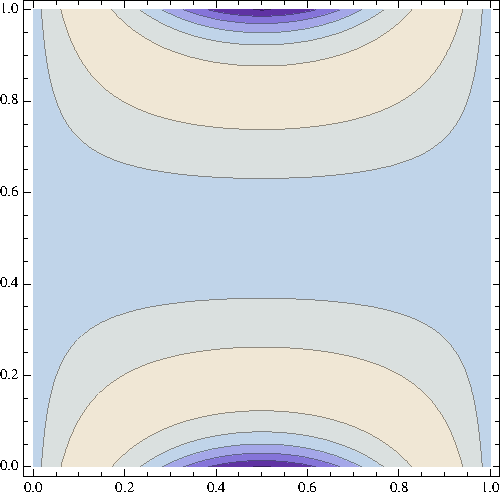
\includegraphics[scale=.7]{mismatchedLnLContourFullParams.pdf}}}
	\put(200,5){\makebox(-0,-150)[l]{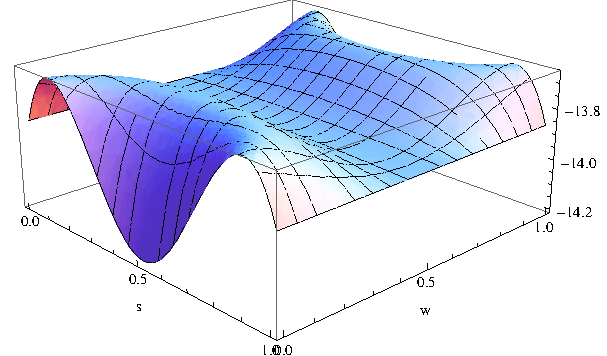
\includegraphics[scale=.7]{mismatchedLnLPlotFullParams.pdf}}}
\end{picture}\\
This is a disturbing set of graphs.  We don't have the likelihood peaking at one point, instead we have pair of curves through the parameter space that form the MLE ridge.

The surface also looks like it has a couple of mirrors placed upon it.  This is a hint that we may be able to reparameterize to avoid considering points of the parameter space that are indistinguishable from one another.





We may notice that $s(1-s)$ is prominent in both terms of our log-likelihood. In fact if we express $1-2s+2s^2$ as $1-2s(1-s)$ then we can see it in even more parts of the equation:
\begin{eqnarray*} 
\ln L(w,s) & = & (n_{00} + n_{11})\ln\left[\left(\frac{1}{4}\right)(1-2s(1-s)) + (\frac{1}{2} -w +w^2) 2s(1-s)\right] + \ldots \\
	& & +  (n_{01} + n_{10})\ln\left[\left(\frac{1}{4}\right)(1-2s(1-s)) + w(1-w)2s(1-s)\right] 
\end{eqnarray*}
This suggests that things will be easier to look at if we substitute a new variable in:
$$ m = 2s(1-s)$$
to get:
\begin{eqnarray*} 
\ln L(w,m) & = & (n_{00} + n_{11})\ln\left[\left(\frac{1}{4}\right)(1-m) + (\frac{1}{2} -w +w^2) m\right] + \ldots \\
	& & +  (n_{01} + n_{10})\ln\left[\left(\frac{1}{4}\right)(1-m) + w(1-w)m\right] 
\end{eqnarray*}
Notice that this replacement actually got rid of $s$ from our equation!

This means that if we knew $m$ and $w$ we could calculate the likelihood without calculating $s$ from $m$.
We say that $\{w,m\}$ is an alternative parameterization of our model, that may be more convenient to work with than $\{w,s\}$.

One great feature of MLE estimation is that we can reparameterize at will. If we estimate  $\hat m$ we can always convert that to a MLE $\hat s$ by solving for the values of $s$ that yield $\hat m$. 
In particular:
\begin{equation}s = \frac{1 \pm \sqrt{1 - 2 m}}{2} \label{EqnSFromM}
\end{equation}

\subsubsection{Reparameterizing constraints}
One {\em caveat} is that our model only allows certain values of $m$, and we must enforce these constraints. 
If we don't, then we can infer values of $m$ that fundamentally disagree with our original model - rather than simply reparameterizing the model we will have changed the predictions that it makes about the data.
To be specific, we know that $s$ is a proportion, so $0\leq s \leq 1$, and we can visualize the values of $m$ in this range:\\
\begin{picture}(200,180)(-0,-160)
	\put(0,5){\makebox(-0,-150)[l]{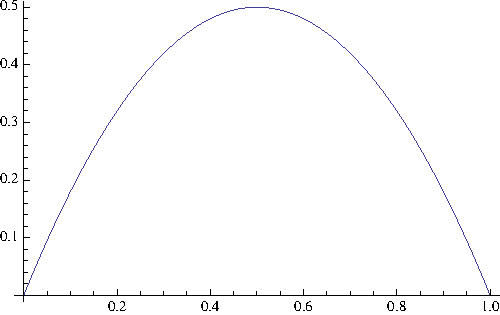
\includegraphics[scale=.7]{mAsFOfs.pdf}}}
\end{picture}\\
The maximum value of $m$ that our model can produce is $0.5$ - this occurs when $s= 0.5$ so the probability of a mismatch is maximized.
In fact if we consult our previous calculations, we will see that what we have named $m$ is simply the probability that one male is strong and the other is weak.
So if we choose to work with $m$ rather than $s$, we must enforce $0\leq m \leq 0.5$ rather than $0\leq s \leq 1$.

Notice (from Eqn \ref{EqnSFromM} or by looking at the plot) that every value of $m$ corresponds to two values of $s$.
Our likelihood may show a preference for some value of $m$, but how will we know which of the two values of $s$ to pick?  We will not know.  
In fact, we are seeing evidence that not all values of $s$ are identifiable based on the experiment that we've performed.  
Even if we had a million trials of two bouts each we would not be able to tell whether $s=0.6$ fits the data better than $s=0.4$.

The reason is that both of these parameter values make the same predictions about the data. 
$s$ only affects the probability of the data ``through'' $m$ - so if two values of $s$ predict the same $m$, then the likelihood will not be able to choose the better value for $s$.
This fact explains some of the symmetry that we saw in the likelihood surface.  If we plot with respect to $w$ and $s$ we less of the ``mirrored'' appearance:\\
\begin{picture}(200,180)(-0,-160)
	\put(0,5){\makebox(-0,-150)[l]{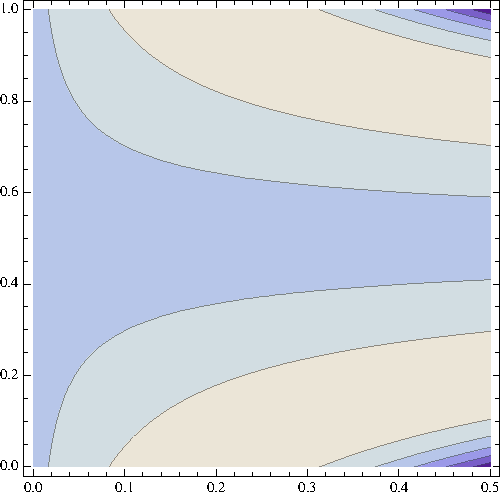
\includegraphics[scale=.7]{mismatchedLnLContourMandW.pdf}}}
	\put(200,5){\makebox(-0,-150)[l]{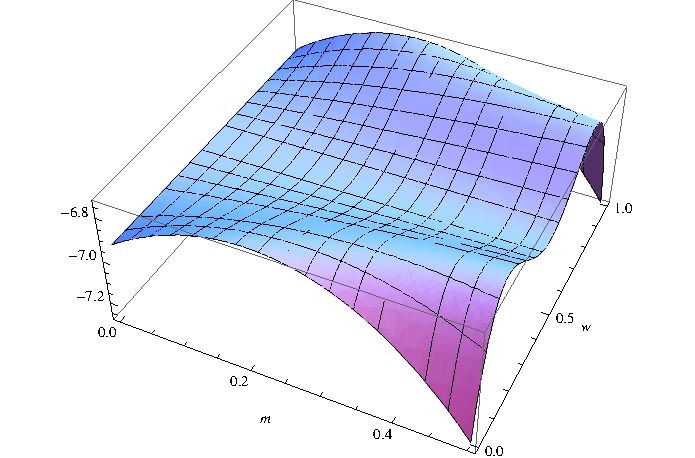
\includegraphics[scale=.7]{mismatchedLnLPlotMandW.pdf}}}
\end{picture}\\
Furthermore we can note that we chose $w$ to represent the probability that the stronger male wins.  This should be at least 0.5 (otherwise he wouldn't be ``stronger''). 
So we can restrict $.5\leq w \leq 1$:\\
\begin{picture}(200,180)(-0,-160)
	\put(0,5){\makebox(-0,-150)[l]{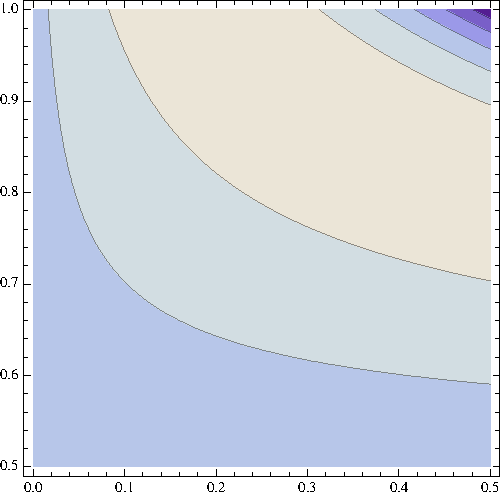
\includegraphics[scale=.7]{mismatchedLnLContourMandWUpper.pdf}}}
	\put(200,5){\makebox(-0,-150)[l]{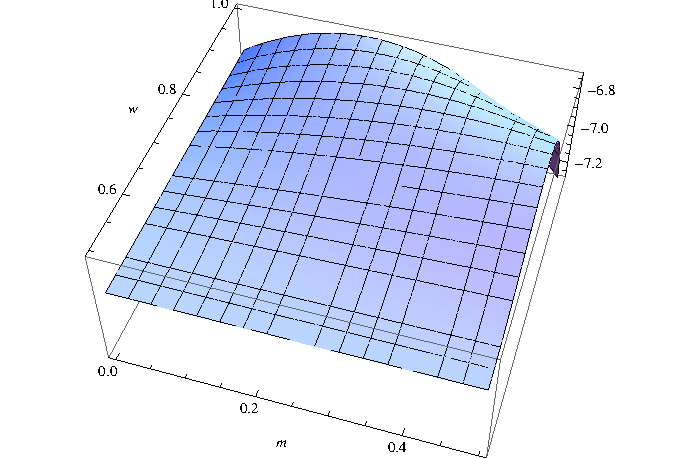
\includegraphics[scale=.7]{mismatchedLnLPlotMandWUpper.pdf}}}
\end{picture}\\
We still have a ridge through the likelihood, but getting rid of the symmetry can make our final answer cleaner to express.  
Note that the non-identifiability of $s$ still exists (we haven't gotten rid of the symmetry in the likelihood function with respect to $s$), but reparameterizing will make our lives easier.

\subsection{Reparameterization again}
We can actually reparameterize a bit further.
If we define a variable:
$$ p = \left(\frac{1}{4}\right)(1-m) + \left(\frac{1}{2} -w +w^2\right)m $$
then we get
\begin{eqnarray*} 
\ln L(p) & = & (n_{00} + n_{11})\ln p  +  (n_{01} + n_{10})\ln\left[\frac{1-2p}{2}\right] \label{defP}
\end{eqnarray*}
This may seem like a big leap, but in it makes sense if you think about it.
$p$ is simply the probability of an outcome in which the same male wins both bouts.  
Given that we arbitrarily labeled the males 0 and 1, it seems intuitive that we should only be concerned with modeling the probability of one male winning both rather than {\em which} male wins a bout.

Furthermore, the discussion on sufficiency revealed that we really only have one relevant quantity that we learn by doing the experiment.
We know $n$ by experimental design.
We observe $n_{00} + n_{11}$, and that single bit of information is the basis of our inference (the other statistic $n_{01} + n_{10}$ is simply $n-n_{00} - n_{11}$).

Given that we only have one ``free'' bit of data, it is not too surprising that we can boil the model down into a one parameter form.

Our model is now analytically tractable:
\begin{eqnarray*} 
\frac{d \ln L(p)}{d p} & = & \frac{(n_{00} + n_{11})}{p}  - \frac{(n_{01} + n_{10})}{\frac{1}{2}-p} \\
0 & = &  \frac{(n_{00} + n_{11})}{\hat p}  - \frac{(n_{01} + n_{10})}{\frac{1}{2}-\hat p} \\
\frac{(n_{01} + n_{10})}{\frac{1}{2}-\hat p}  & = &  \frac{(n_{00} + n_{11})}{\hat p} \\
(n_{01} + n_{10})\hat p  & = &  (\frac{1}{2}-\hat p)(n_{00} + n_{11})\\
(n_{01} + n_{10}+ n_{00} + n_{11})\hat p  & = &  \frac{n_{00} + n_{11}}{2} \\
(n)\hat p  & = &  \frac{n_{00} + n_{11}}{2} \\
\hat p  & = &  \frac{n_{00} + n_{11}}{2n} = 0.3 \\
\end{eqnarray*}
Once again, we must pay attention to the constraints on our new parameterization.
Plotting (or examining the Eqn \ref{defP}) helps us see that $p$ gets larger as either $w$ or $m$ get larger:\\
\begin{picture}(200,180)(-0,-160)
	\put(0,5){\makebox(-0,-150)[l]{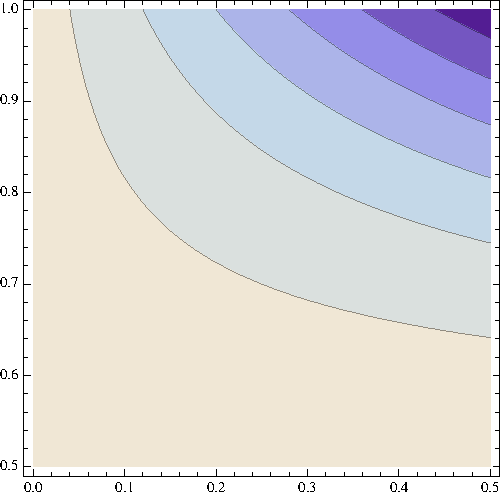
\includegraphics[scale=.7]{pContour.pdf}}}
	\put(200,5){\makebox(-0,-150)[l]{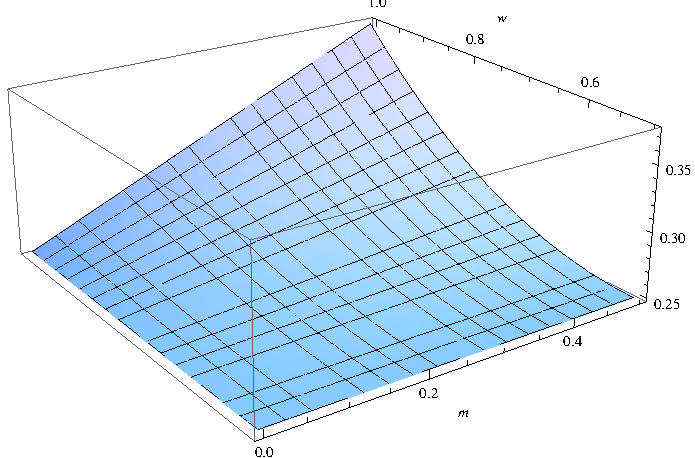
\includegraphics[scale=.7]{pPlot.pdf}}}
\end{picture}\\
Thus the smallest value of $p$ occurs when $m=0$ and $w=.5$. At this point $p = .25$.
The largest value attainable value of $p$ occurs at $p=3/8$ when $m=.5$ and $w=1$.

Fortunately, $\hat p$ that we calculated falls in this range, so we have found a value that maximizes the likelihood and still fits our model.

We can translate back to $w$ and $m$ via:
\begin{eqnarray*} 
	\hat m = \frac{\hat p - .25}{.25 - \hat w + \hat w^2} \\
	\hat w = \frac{\hat m + \sqrt{(4\hat p - 1)\hat m}}{2 \hat m} \\
\end{eqnarray*} 
But these are not very satisfying because each MLE corresponds to a range of values (depending on the MLE of the other parameter).

Fortunately analyzing how $w$ and $m$ interact reveals that the range of values that are on the MLE ridge follow a convenient form:
$$ \hat w_{m=.5}\leq\hat w \leq 1$$
where $\hat w_{m=.5}$   is the MLE of $w$ when $m$ is forced to its maximum value of 0.5:
\begin{eqnarray*} 
	\hat w_{m=.5} & = & .5 + \sqrt{(2\hat p - .5)} \\
\end{eqnarray*} 
So
$$ .5 + \sqrt{(2\hat p - .5)}\leq\hat w \leq 1$$

The lowest MLE of $m$ occurs when $w=1$, so:
$$ \hat m_{w=1} \leq \hat m \leq 0.5 $$
\begin{eqnarray*} 
	\hat m_{w=1} & = &\frac{\hat p - .25}{.25 - 1 + 1} \\
	& = & 4 \hat p - 1
\end{eqnarray*} 
So
$$ 4 \hat p - 1 \leq \hat m \leq 0.5 $$

For our problem, $\hat p = 0.3$ so:
\begin{eqnarray*} 
	0.816227766016838 & \leq \hat w \leq & 1 \\
	.2 & \leq \hat m \leq & .5
\end{eqnarray*} 
These broad ranges are seen by plotting the profile of the log-likelihood with respect to each parameter (first $w$ then $m$):\\
\begin{picture}(200,180)(-0,-160)
	\put(0,5){\makebox(-0,-150)[l]{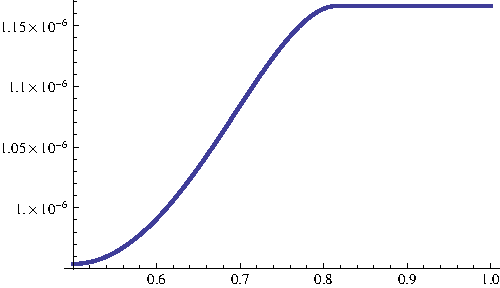
\includegraphics[scale=.7]{wProfile}}}
	\put(200,5){\makebox(-0,-150)[l]{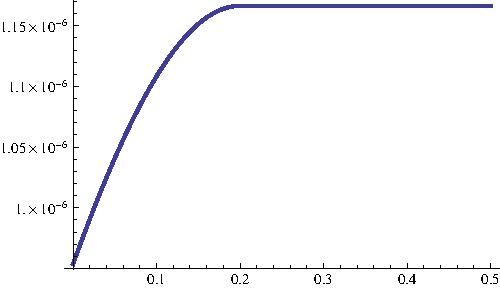
\includegraphics[scale=.7]{mProfile.pdf}}}
\end{picture}\\

We can use the LRT to construct the confidence interval on $p$ and then translate that into statements about $w$ or $m$ (or even back to $s$ by converting the statements about $m$ into terms of $s$).

\bibliography{phylo}
\end{document}  
